\documentclass[oneside,numbers,english]{ezthesis}

\usepackage{setspace}
\usepackage{graphicx}
\usepackage{url}
\usepackage{float}
\usepackage{fancybox}
\usepackage{framed,color}
\usepackage{listings}
\usepackage{color}

\definecolor{dkgreen}{rgb}{0,0.6,0}
\definecolor{gray}{rgb}{0.5,0.5,0.5}
\definecolor{mauve}{rgb}{0.58,0,0.82}
\definecolor{shadecolor}{rgb}{1,0.8,0.3}

\lstset{frame=tb,
  language=Java,
  aboveskip=3mm,
  belowskip=3mm,
  showstringspaces=false,
  columns=flexible,
  basicstyle={\small\ttfamily},
  numbers=none,
  numberstyle=\tiny\color{gray},
  keywordstyle=\color{blue},
  commentstyle=\color{dkgreen},
  stringstyle=\color{mauve},
  breaklines=true,
  breakatwhitespace=true
  tabsize=1
}


%% # Opciones disponibles para el documento #
%%
%% Las opciones con un (*) son las opciones predeterminadas.

%% Formato de las referencias bibliogr'aficas:
%%   numbers          - numeradas, p.e. [1]
%%   authoryear (*)   - por autor y a'no, p.e. (Newton, 1997)
%%


%% # Datos del documento #

\author{Jos\'e Antonio Magro Cort\'es}
\title{BigData. Integrating NoSQL Technologies into Virtual Observatory}
\degree{Master's Thesis}
\supervisor{Juan de Dios Santander Vela}
\institution{Universidad de Granada / Instituto de Astrof\'isica de Andaluc\'ia}
\faculty{}
\department{}

%% # M'argenes del documento #
%% 
%% Quitar el comentario en la siguiente linea para ajustar los m'argenes del
%% documento. Leer la documentaci'on de "geometry" para m'as informaci'on.

%\geometry{top=40mm,bottom=33mm,inner=40mm,outer=25mm}


%% El siguiente comando agrega ligas activas en el documento para las
%% referencias cruzadas y citas bibliogr'aficas. Tiene que ser *la 'ultima*
%% instrucci'on antes de \begin{document}.
\hyperlinking
\begin{document}

%% # Portada de la tesis #
%% ## Construye tu propia portada ##
%% 
%% Una portada se conforma por una secuencia de "Blocks" que incluyen
%% piezas individuales de informaci'on. Un "Block" puede incluir, por
%% ejemplo, el t'itulo del documento, una im'agen (logotipo de la universidad),
%% el nombre del autor, nombre del supervisor, u cualquier otra pieza de
%% informaci'on.
%%
%% Cada "Block" aparece centrado horizontalmente en la p'agina y,
%% verticalmente, todos los "Blocks" se distruyen de manera uniforme 
%% a lo largo de p'agina.
%%
%% Nota tambi'en que, dentro de un mismo "Block" se pueden cortar
%% lineas usando el comando \\
%%
%% El tama'no del texto dentro de un "Block" se puede modificar usando uno de
%% los comandos:
%%   \small      \LARGE
%%   \large      \huge
%%   \Large      \Huge
%%
%% Y el tipo de letra se puede modificar usando:
%%   \bfseries - negritas
%%   \itshape  - it'alicas
%%   \scshape  - small caps
%%   \slshape  - slanted
%%   \sffamily - sans serif
%%
%% Para producir plantillas generales, la informaci'on que ha sido inclu'ida
%% en el archivo principal "tesis.tex" se puede accesar aqu'i usando:
%%   \insertauthor
%%   \inserttitle
%%   \insertsupervisor
%%   \insertinstitution
%%   \insertdegree
%%   \insertfaculty
%%   \insertdepartment
%%   \insertsubmitdate

\begin{titlepage}

%\begin{picture}(0,0)

\includegraphics[width=4cm,height=4cm]{images/logo_ugr.jpg}

\includegraphics[width=4cm,height=4cm]{images/logo_iaa.png}
%\end{picture}


  \TitleBlock{\scshape\insertinstitution}
  \TitleBlock[\bigskip]{\scshape\insertfaculty}
  \TitleBlock{\Huge\scshape\inserttitle}
  \TitleBlock{\scshape
    M\'aster en M\'etodos y T\'ecnicas Avanzadas en F\'isica \\ Trabajo Fin de M\'aster presentado por \insertauthor}
  \TitleBlock{\insertsubmitdate}
  \TitleBlock[\bigskip]{\insertdepartment}
\end{titlepage}

%% Nota 1:
%% Se puede agregar un escudo o logotipo en un "Block" como:
%%   \TitleBlock{\includegraphics[height=4cm]{escudo_uni}}
%% y teniendo un archivo "escudo_uni.pdf", "escudo_uni.png" o "escudo_uni.jpg"
%% en alg'un lugar donde LaTeX lo pueda encontrar.

%% Nota 2:
%% Normalmente, el espacio entre "Blocks" se extiende de modo que el
%% contenido se reparte uniformemente sobre toda la p'agina. Este
%% comportamiento se puede modificar para mantener fijo, por ejemplo, el
%% espacio entre un par de "Blocks". Escribiendo:
%%   \TitleBlock{Bloque 1}
%%   \TitleBlock[\bigskip]{Bloque2}
%% se deja un espacio "grande" y de tama~no fijo entre el bloque 1 y 2.
%% Adem'as de \bigskip est'an tambi'en \smallskip y \medskip. Si necesitas
%% aun m'as control puedes usar tambi'en, por ejemplo, \vspace*{2cm}.





\tableofcontents

%% # Prefacios #
%\prefacesection{Acknowledgments}


\pagenumbering{Roman}
\begin{flushright}

\textit{En primer lugar debo reconocer la deuda que tengo con mi tutor, el Dr. Juande Santander, por aceptarme como alumno, por compartir sus conocimientos conmigo, por sus revisiones, anotaciones y correcciones. Por su disponibilidad a pesar de la distancia, de la diferencia horaria y del resto de circunstancias. Por la pasi\'on que le pone a su trabajo. !`Gracias maestro!}


\textit{\newline A la Dra. Maribel Tercedor, porque sin ella preverlo, hace 15 a\~{n}os una frase suya cambi\'o mi rumbo laboral. Este bandazo acad\'emico se lo debo a ella.}


\textit{\newline A Mamen, Antonio y Alejandro por permitir embarcarme en esta locura a pesar de las horas que les iba a robar y por aportar la cordura necesaria para compatibilizar trabajo, estudios y familia.}


\textit{\newline A mis padres, por contagiarme el virus de la curiosidad a base de comprarme libros y m\'as libros y darme toda clase de facilidades.}


\textit{\newline A mis abuelos: el \'exito de vuestra lucha se refleja en momentos como \'este, a pesar de que últimamente algunos se empe\~{n}an en destruir vuestro legado. No lo conseguir\'an.}


\textit{\newline A Laura y Mar\'ia del Mar, compa\~{n}eras, por las risas entre clase y clase (y fuera de ellas) y por haber ayudado a este \emph{intruso}. Llegar\'eis lejos, os lo merec\'eis.} 

\end{flushright}


%\begin{abstract} Abstract. \end{abstract}


%% # 'Indices y listas de contenido #
\listoffigures
\listoftables

%% # Cap'itulos #
\chapter{Overview}

\pagenumbering{arabic}

The volume of data produced at some science centers presents a considerable processing challenge. At CERN, for instance, several hundred million times per second, particles collide inside LHC. Each collision generates particles that often decay in complex ways into more particles. The pass of particles are recorded through a detector that sends the data for digital reconstruction. Physicists have then to browse through petabytes of data annually yielded to determine if the collisions have thrown up any interesting information. \newline

CERN, like many other science centers, does not have the computing or financial resources to manage all of the data on its site, so it moved into the grid to share the load with computing centers around the world. The Worldwide LHC Computing Grid is a distributed system which gives over 8000 physicists near real-time access to LHC data.  \newline

So we could think that current deployed technologies are maybe obsolete and a new rethink should be made. If CERN (but not just CERN as we will discuss later) has changed its storage policy (leaving behind the classic client-server model), why not change the way the data are accessed?  \newline

Almost a decade after E. Codd published his famous relational model paper, the relational database management systems (RDBMS) have been the \textit{de facto} tools. Today, non-relational, cloud, or the so-called NoSQL databases are growing rapidly as an alternative model for database management. Often more features apply such as schema-less, easy replication feature, simple API, eventually consistent / BASE (not ACID), a huge amount of data (big data) and more. \newline

In this work, we give a short overview of big data problem and present an alternative, using one of the NoSQL databases (today, the volumes of data that can be handled by NoSQL systems exceed what can be handled by the biggest RDBMS) freely available, to offer a different way of challenging some of these problems, always operating inside VO frame.
\chapter{Big Data challenges in astronomy} % \chapter{Astronomy Big Data}
\label{theproblem}

Astronomical datasets are growing at an exponential rate: the next generation of telescopes will collect data at rates of
several terabytes % terabytes
per day. This data
deluge % , now and int the future,
presents some critical challenges for the way astronomers
can
get new knowledge from their data.
These extremely large datasets, or datasets with high data rates, are commonly known as
\emph{Big Data}.

Big Data are high-volume, high-velocity, and/or high-variety information assets that require new forms of processing to enable enhanced
decision making\footnote{For instance, fast follow up of transients in the data collected by the LSST.}, % decision making,
insight discovery and process optimization. Examples of Big Data
outside of astronomy
include information
systems
such as Web search results, electronic messages (e.g. SMS, email and instant messages), social media postings, pictures, videos, 
or large web % and 
system log data.
% However, it can also include cash transactions, check images, receipts and other transactional information depending on the source of the information.
These situations require the % This situation requires
processing of terabytes and even petabytes of data. This is achieved by
means of
distributed, segmented
processing.
% This is one of major reasons for the power of Web companies such as Google, Amazon or social networks like Facebook and Twitter.
% Relational databases

Relational Database Systems (RDBMS)
are found to be inadequate in distributed processing involving very large number of servers and handling Big Data applications, due to the limitations of query speed, storage size, and scalabilty inherent to the tasks of keeping relationships between database tables, atomicity of transactions, and the storage layout of data in disk.

% In this chapter, we make an overview of some of the greatest telescopes and the amount of data they acquire and store.

In the next sections, we will review some of the current and future challenges for astronomical data processing, which justify the search for NoSQL solutions for astronomical data sharing.

% \section{Atacama Large Millimiter Array}
\section{The Atacama Large Millimetre/Submillimetre Array}

The Atacama Large Millimetre/Submillimetre Array (ALMA) % ALMA
is a worldwide project, % ; the synthesis of early visions of astronomers in its three partner communities: Europe, North America and Japan. It is a fusion of ideas, with its roots in three astronomical projects: the Millimeter Array (MMA) of the United States, the Large Southern Array (LSA) of Europe, and the Large Millimeter Array (LMA) of Japan.
built cooperatively by the European Southern Observatory (ESO), the National Radio Astronomical Observatory (NRAO) of the United States of America, and the National Astronomical Observatory of Japan (NJAO), in collaboration with the Academia Sinica of Taiwan.

 \begin{figure}[tb]
 \centering
 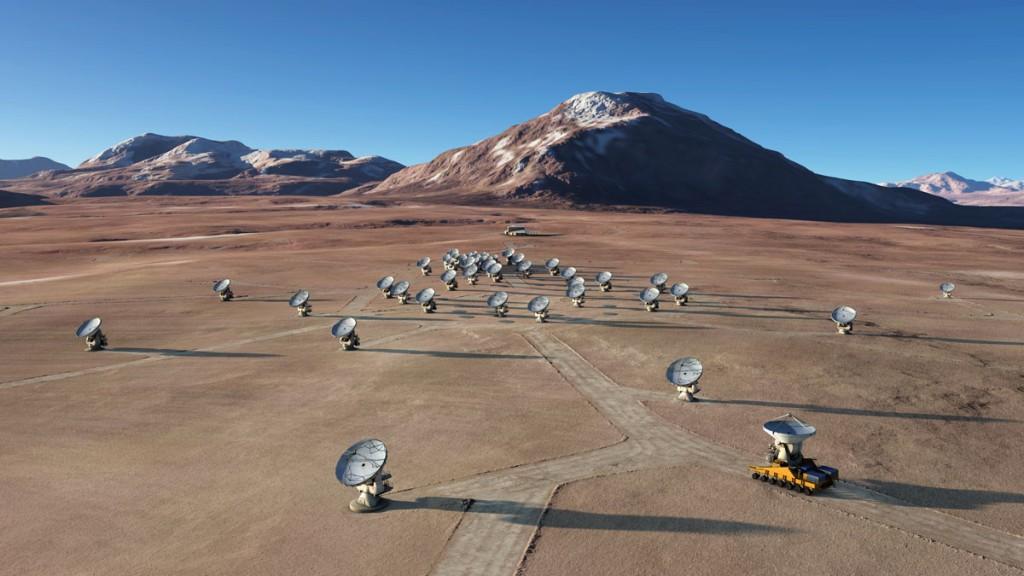
\includegraphics[width=\textwidth]{images/alma.jpg}
 % \caption{ALMA dishes in Atacama Desert}
 \caption{Artist's impression of ALMA dishes at the Chajnantor plateau, in the Atacama Desert}
 \end{figure}


ALMA
% is an instrument that
consists of a giant array of
sixty-six
12~m antennas with baselines up to
16~km,
and an additional compact array of
7~m
and
12~m antennas to greatly enhance ALMA's ability to image extended targets, located on the Chajnantor plateau at 5000m altitude.

%The design of
ALMA is driven by three key science goals:

\begin{itemize}

\item Detecting spectral line emission from CO in a normal galaxy like the Milky Way at a redshift of $z=3$, in less than 24 hours.

\item Imaging the gas kinematics in protostars and in protoplanetary disks around young Sun-like stars in the nearest molecular clouds
(150~pc).

\item Providing precise high dynamic range images at an angular resolution of
0.1~arc-seconds
\end{itemize}

In order to accomplish those goals,
% Initially, it will
ALMA will initially 
observe at wavelengths in the range 3~mm to
400~$\mu{}$m
(84 to 720~GHz). The antennas can be moved around, in order to
provide different % form arrays with different distributions of 
baseline lengths. More extended
configurations % arrays
% will
give
higher % high
spatial resolution,
while
more compact arrays give better sensitivity for extended sources. In addition to the array of
12~m
antennas, there is the Atacama Compact Array (ACA), used to image large scale structures that are not well sampled by the ALMA
12~m
array, consisting of twelve
7~m
antennas and four
12~m
antennas. 


The current ALMA Archive design allows for a maximum
raw
data rate of 64 MB/s and an average data rate
of 6.4 MB/s, which produces the long-term storage capacity of approximately 200 TB/year. The
ALMA correlators can
generate % producing a
data
up to 1000 MB/s. 
Reduced ALMA datacubes will have thousands of channels with millions of pixels, supporting multiple polarizations, and will range from tens to hundreds of gigabytes.

% \section{Square Kilometer Array}
\section{The Square Kilometre Array} % (fold)
\label{sec:the_square_kilometre_array}
The Square
Kilometre % Kilometer
Array\urlnote{http://www.skatelescope.org/} (SKA) % Array (SKA)
is a global science and engineering project led by the SKA Organization, a not-for-profit company with its headquarters at Jodrell Bank Observatory, near Manchester. When construction starts in 2016 (according to
the official schedule\urlnote{http://www.skatelescope.org/the-project/project/}) % schedule)
in Australia and in Southern Africa, thousands of linked radio wave receptors will be located to combine the signals from the antennas in each region creating a telescope with a collecting area equivalent to a dish with an area of about one square kilometer to discover how the first stars and galaxies formed after the Big Bang, how galaxies have evolved and the nature of gravity. It comprises:

\begin{itemize}
\item An array of dish receptors in eight African countries. 
\item An array of mid frequency aperture arrays in the Karoo. 
\item A smaller array of dish receptors and an array of low frequency aperture arrays in the Murchison Radio-astronomy Observatory in Australia.
\end{itemize}

 \begin{figure}[tb]
 \centering
 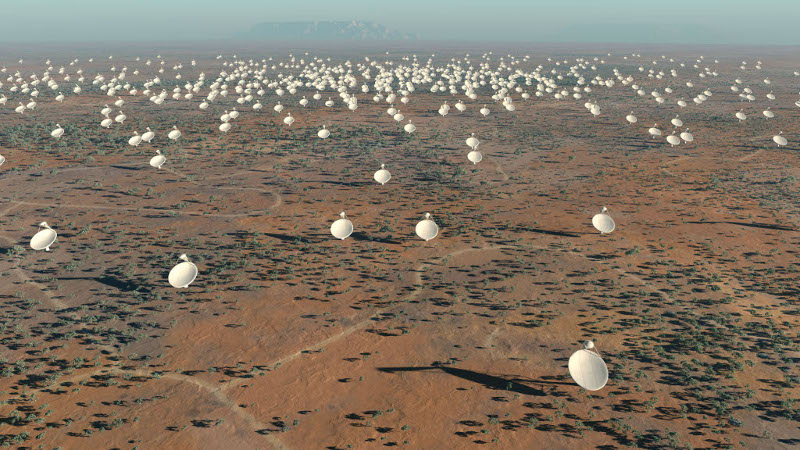
\includegraphics[width=\textwidth]{images/ska.jpg}
 \caption{Artist's impression of the SKA dishes. Credit: SKA Organisation/TDP/DRAO/Swinburne Astronomy Productions}
 \end{figure}

% NOTA: Si fuera posible, cambiar por algo del Science Data Processor.

Some relevant figures and facts about SKA:

\begin{itemize}

\item The data collected by the SKA in a single day would take nearly two million years to playback on an ipod.
\item The SKA central computer will have the processing power of about one hundred million PCs.
\item The SKA will use enough optical fibre to wrap twice around the Earth.
\item The dishes of the SKA will produce 10 times the global internet traffic.
\item The SKA will generate enough raw data to fill 15 million 64 GB iPods every day.
\item SKA will be able to detect an airport radar on a planet 50 light years away.

\end{itemize}

% section the_square_kilometre_array (end)



\section{Murchison Widefield Array} % (fold)
\label{sec:murchison_widefield_array}

The Murchison Widefield Array is
one of % NOTA: ASKAP está muy cerca, no querría pillarme los dedos
the first Square Kilometre Array precursor to enter full operations, generating a huge amount of information that needs to be stored for later retrieval by scientists. To store the data generated by the MWA three 1 TB hard drives every two hours are needed (it will store about 3 Petabytes at the Pawsey Center each year), so the
problem is not % isn not
just a matter of storing the observations but how to distribute them from the MWA team in remote places, like
the MIT, % MIT,
Victoria University of Wellington in New Zeahland and India. 

According to Professor Andreas Wicenec, from The University of Western Australia node of the International Centre for Radio Astronomy Research (ICRAR),
the MWA % SKA
% NOTA: cambiar verbos, y asegurar que hay un link o cita que justifique la cita literal
has ``now have more than 400 megabytes per second of MWA data streaming along the National Broadband Networ¡k from the desert 800 km away''. Data travels through a 10 gigabit per second connection between the Murchison Radio-astronomy Observatory (MRO) and
Geraldton\urlnote{http://www.skatelescope.org/news/pawsey-centre/}.

The data are not obviously intended to be fully available for everybody at every time: for instance, MIT researchers are interested in the early universe so filtering techniques to control what data is copied from the Pawsey Center archive to the MIT machines are used. By 2013, more than 150 TB of data had been transferred automatically to the MIT store, with a stream of up to 4 TB a day increasing that value. 

% section muchison_widefield_array (end)



% \section{Large Synoptic Survey Telescope}
\section{Large Synoptic Survey Telescope} % (fold)
\label{sec:large_synoptic_survey_telescope}

The Large Synoptic Survey Telescope (LSST) is a new kind of telescope whose widefield of view allows it to observe large areas of the sky at once. It can take almost 1000 panoramic images each night,
covering % it can cover
the sky twice a week. Data from
the
LSST will be used to create a 3D map of the Universe with unprecedented depth and detail. Plans for sharing the data from LSST with the public are really ambitious, as it is intended that anyone with a
personal computer % PC
will be able to % can
fly through the Universe, zooming past objects a hundred million times fainter than
what
can be observed with the human eye. 

Some of the institutional members\footnote{See \url{http://lsst.org/lsst/about/members}} are Google, Caltech, Harvard-Smithsonian Center for Astrophysics, Fermi National Accelerator Laboratory or STSI.  


LSST observing will produce about 30 TB per night, leading to a total database over the ten years of operations of 60 PB for the raw data, and 30 PB for the catalog database, that will be processed using 100 TFlops. The data will be sent over existing optical fiber links from Chile to the U.S. 

Currently finishing the design and development stages, it is expected to start operating in 2022.

% section large_synoptic_survey_telescope (end)
\chapter{The Virtual Observatory} % (fold)
\label{cha:the_virtual_observatory}


The International Virtual Observatory Alliance\urlnote{http://www.ivoa.net/}
(IVOA) was formed in 2002 with the aim to
\emph{``facilitate the international coordination and collaboration necessary for the development and deployment of the tools, systems and organizational structures necessary to enable the international utilization of astronomical archives as an integrated and interoperating virtual observatory.''}
The IVOA now comprises programs from several countries and intergovernmental organizations like ESA and ESO. 

The IVOA focuses on the development of standards and encourages their implementation for the benefit of the worldwide astronomical community.
As a result, a federation of lightly-coupled, interoperable web-services provide astronomers with data from multiple data archives and catalogues.
Working Groups are constituted with cross-program membership in those areas where key interoperability standards and technologies have to be defined and agreed upon. The Working Groups develop standards using a process modeled after the World Wide Web Consortium, in which Working Drafts progress to Proposed Recommendations and finally to Recommendations. Recommendations may ultimately be endorsed by the Virtual Observatory Working Group of Commission 5 (Astronomical Data) of the International Astronomical Union. The IVOA also has Interest Groups that discuss experiences using VO technologies and provide feedback to the Working Groups. 

In this section we are not going to make a deep study of the Virtual Observatory techniques, technologies, protocols and interfaces, just those needed and selected to explain our proposal of including NoSQL into VO. Bearing in mind that the problem we are trying to address is data modelling, we will just make an overview of those aspects related with our work.

\section{ObsTAP} % (fold)
\label{sec:obstap}


A data model is a description of the objects represented by a computer system with their properties and relationships, a logical model detailing the decomposition of a complex dataset into simpler elements, like a collection of concepts and rules used in defining data model. 

In 2011 IVOA proposed a new recommendation: Observation Data Model Core
Components~\cite{2011arXiv1111.1758L}
and its Implementation in the Table Access
Protocol~\cite{2010tap..irec.....D}.
That document was intended to be a description of the interface which integrated the data modeling and data access aspects in a single service: ObsCore data model + Table Access Protocol = ObsTAP.

\subsection{ObsCore Components Data Model}

Its aim is to get the generic data model for the metadata necessary to describe any astronomical observation. In the IVOA recommendation, the data are described using
% UML.
the Unified Modelling Language~\cite{Burkhardt:1997:UML} (UML).

\subsection{Table Access Protocol}

TAP defines a Web service for accessing tables containing astronomical catalogues. TAP is the protocol which underlies in the process of posing a query against a data source (or several data sources). The result of a query is a table, usually a VOTable.\footnote{Support for VOTable output is mandatory, while other formats may be available.}  

Queries which use TAP protocol can be made through several clients, like:
\begin{itemize}
\item TOPCAT\urlnote{http://www.star.bris.ac.uk/~mbt/topcat/}
\item TAPHandle\urlnote{http://saada.unistra.fr/taphandle/}
is a TAP client
 which operates fully within the Web browser
\item The TAP shell\urlnote{http://vo.ari.uni-heidelberg.de/soft/tapsh}, a command line interface to querying TAP servers, complete with metadata management and command line completion.
\item The GAVO VOTable library\urlnote{http://docs.g-vo.org/DaCHS/votable.html}, which allows embedding TAP queries in Python.
\end{itemize}

The types of queries implemented by TAP are:

\begin{itemize}
\item data queries, where the query result is directly the science data to be operated upon;
\item metadata queries, where the query result is metadata of the datasets, the archival service, or both; and
\item Virtual Observatory Support Interface (VOSI) queries, which provide information on the different TAP service capabilities.
\end{itemize}


TAP includes support for multiple query languages, including queries specified using the Astronomical Data Query Language (ADQL; see~\cite{2008adql.ivoav0910O}) and the Parameterised Query Language~\cite{IVOA-Data-Access-Layer-Working-Group:2009lr} (PQL, under development). Other query languages are also supported, and this mechanism allows developments outside the IVOA to be used without modifying the TAP specification. Finally, it also includes support for both synchronous and asynchronous queries. Special support is provided for spatially indexed queries using the spatial extensions in ADQL. 

Listing~\ref{lst:adqlsample} shows an ADQL sample query: a crossmatch between a user-uploaded catalog (\texttt{TAP\_UPLOAD.T1}), and
the Third US Naval Observatory CCD Astrograph Catalog\urlnote{http://www.usno.navy.mil/USNO/astrometry/optical-IR-prod/ucac} (UCAC3) % UCAC
catalog, compensating the fit for proper motion.

\begin{lstlisting}[float,language=SQL,caption={ADQL sample query: the results will be a crossmatch between a user-uploaded catalog, and the UCAC3 catalog, compensating the fit for proper motion.},label=lst:adqlsample]
SELECT 
 u.raj2000+d_alpha+d_pmalpha/cos(radians(u.dej2000))*(u.epoch-2000) AS ra_icrs,
 u.dej2000+d_delta+d_pmdelta*(u.epoch-2000) AS de_cicrs,
 u.pmra+d_pmalpha AS pmra_icrs,
 u.pmde+d_pmdelta AS pmde_icrs,
 u.*
FROM
  TAP_UPLOAD.T1 AS u
  JOIN ucac3.icrscorr AS c
  ON (c.alpha=FLOOR(u.raj2000)+0.5 and c.delta=FLOOR(u.dej2000)+0.5)
\end{lstlisting}

% section obstap (end)

\section{Flexible Image Transport System} % (fold)
\label{sec:flexible_image_transport_system}


The
Flexible Image Transport System (FITS) is an open standard defining a digital file format useful for storage, transmission and processing of scientific and other images. FITS is the most commonly used digital file format in astronomy. Unlike many image formats, FITS is designed specifically for scientific data and hence includes many provisions for describing photometric and spatial calibration information, together with image origin metadata. The FITS format was first standardized in 1981; it has evolved gradually since then, and the most recent version (3.0) was standardized in 2008. 
  
FITS is also often used to store non-image data, such as spectra, photon lists, data cubes, or even structured data such as multi-table databases. A FITS file may contain several extensions, and each of these may contain a data object. For example, it
could be % is
possible to store
X-ray % x-ray
and infrared exposures in the same file. 
 
FITS support is available in a variety of programming languages that are used for scientific work, including C, C++, C\#, Fortran, IDL, Java, Mathematica, MatLab, Perl, PDL, or Python. 
 
Image processing programs such as GIMP can generally read simple FITS images, but cannot usually interpret complex tables and databases.

\subsection{FITS Data Format}

Each FITS file consists of one or more headers containing ASCII card images that carry keyword/value pairs, interleaved between data blocks. The keyword/value pairs provide information such as size, origin, coordinates, binary data format, free-form comments, history of the data, and anything else the creator desires. In more technical terms, a FITS file is comprised of parts called Header Data Units (HDU), being the first HDU called primary HDU o primary array. This array can contain a 1-999 dimensional array. A typical primary array could contain a 1D spectrum, 2D image or 3D data cube. Any number of HDU can follow the main array, and are called FITS extensions. Currently, three different extensions can be defined:

\begin{itemize}
\item Image extension, a 0-9999 dimensional array of pixels, which begins with \texttt{XTENSION = `IMAGE'}
\item ASCII table extension which stores tabular data in ASCII formats. They begin with \texttt{XTENSION = `TABLE'}
\item Binary table extension stores tabular data in binary representation. Headers start with \texttt{XTENSION = `BINTABLE'}
\end{itemize}

Besides, there are additional type of HDU called random groups, but only used for radio interferometry.
      
\begin{figure}[tb]
\centering
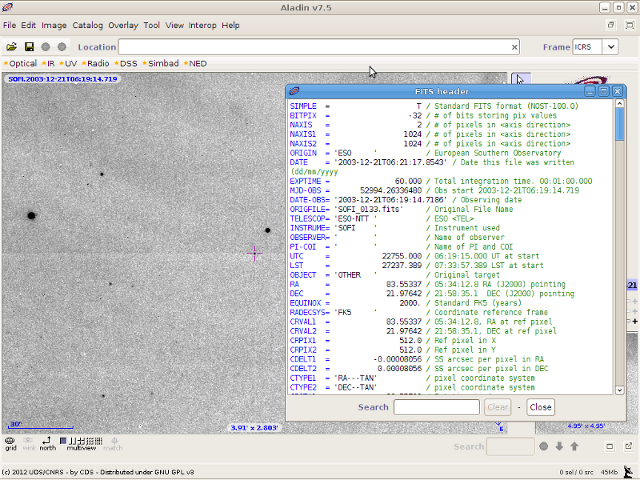
\includegraphics[width=11cm,height=8cm]{images/fits_header.png}
\caption{Viewing a FITS header in Aladin}
\end{figure}

% section flexible_image_transport_system (end)

\section{OpenCADC} % (fold)
\label{sec:opencadc}

OpenCADC (Canadian Astronomy Data Center) is a Virtual Observatory, used in ALMA Science Archive (for this reason is included in this chapter) tool which comprises several projects\footnote{We do not enumerate all of them here, for a full list, go to \url{https://code.google.com/p/opencadc/source/browse}}:

\subsection{Universal Worker Service}

The Universal Worker Service (UWS) pattern defines how to build asynchronous (the client does not wait for each request to be fulfilled; if the client disconnects from the service then the activity is not aborted), stateful (the service remembers results of a previous activity), job-oriented (the rules for setting and arranging the parameters for a job is called Job Description Language- JDL) services.

\begin{figure}[tb]
\centering
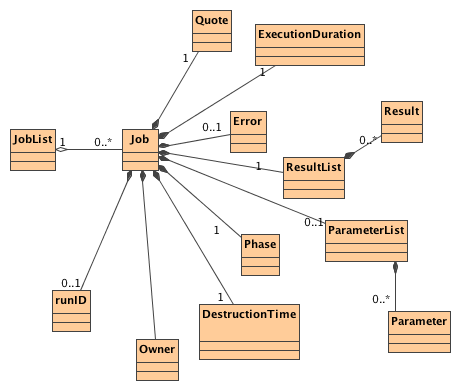
\includegraphics[width=11cm,height=8cm]{images/Class_Diagram__UWS__UWSObjects.png}
\caption{Class diagram representing UWS objects}
\end{figure}

When the execution starts, the job can adopt several states. The phases are the following:



\begin{figure}[tb]
\centering
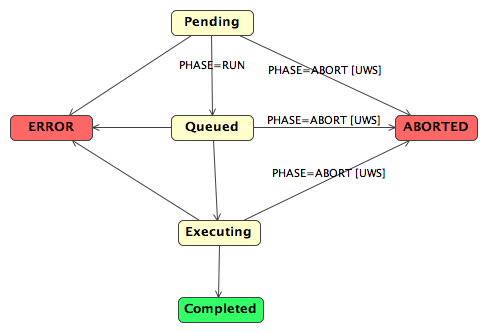
\includegraphics[width=11cm,height=8cm]{images/UWSStates.png}
\caption{Universal Worker Server Job states}
\end{figure}

Now, we make a subtle description of the structure of the code relating UWS in OpenCADC (the cadcUWS Library), the section of the code provides Job class and plugin architecture, servlet with UWS async and sync behaviour.

\subsubsection{JobManager}

Responsible for job control.

\subsubsection{JobPersistence}

In charge of storing and retrieving Job state.

\subsubsection{JobExecutor}

It executes every job in separated threads.

\subsubsection{JobRunner}

The code that actually executes the job.


\subsection{cadcTAP Library}

The cadcTAP library is responsible of async and sync queries, where QueryRunner implements JobRunner. It also contains TAP\_SCHEMA\footnote{TAP services try to be self-describing about what data they contain. They provide information on what tables they contain in special tables in TAP\_SCHEMA}
Data Definition Language\footnote{In RDBMS, the Data Definition Language is the language that allows for the creation of tables, fields, and data types.} (DDL) % DDL
statements and is used by query parser to validate table and column usage.

\subsubsection{TapQuery Interface}

It has a separate implementation for each LANG (e.g. \texttt{LANG=ADQL}) specified and processess the query to local SQL.

\subsubsection{SqlQuery}

When code states \texttt{LANG=SQL}, it implements TapQuery and fully navigates it (\texttt{FROM}, \texttt{WHERE} and \texttt{HAVING} clauses).

\subsubsection{AdqlQuery}

Same as before when \texttt{LANG=ADQL}.

\subsubsection{Plugins}

\begin{itemize}
\item UploadManager
\item TableWriter
\item FileStore
\end{itemize}


\subsubsection{QueryRunner}

It implements JobRunner and sets Job state, find DataSource and uses TapSchema, UploadManager, TapQuery and TableWriter.

% section opencadc (end)



% chapter the_virtual_observatory (end)

\chapter{Non-relational DBMS inside VO}

Typically, modern relational databases have shown little efficiency in certain applications using intensive data, like indexing of a large number of documents, sites rendering with high traffic, and streaming sites. Typical RDBMS implementations are tuned either for small but frequent reads and writes or a large set of transactions that have few write accesses. On the other hand NoSQL DB are optimized for read and append operations, and perform outstandingly where a relational DB would slow down. They are especially fast when large amounts of data have to be queried and if we consider that speed is more important than consistency. \newline

IVOA has a standard called Astronomical Data Query Language (ADQL) that users do not necessarily need to know, because he can pose a query with a GUI, as long as the query is translated into standard ADQL. The receiving service likewise converts the standard ADQL into whatever its own database servers need, but always inside relational model. For the reasons stated in chapter \ref{theproblem}, we propose the use of a different approach, the NoSQL technology.


\section{NoSQL}

A non-relational database just stores data without explicit and structured mechanisms to link data from different buckets to one another. \newline

NoSQL implementations used in the real world include 3TB Digg green markers (indicated to highlight the stories voted by others in the social network), the 6 TB of "ENSEMBLE" European Commission database used in comparing models and air quality, and the 50 TB of Facebook inbox search. \newline

NoSQL architectures often provide limited consistency, such as events or transactional consistency restricted to only data items. Some systems, however, provide all guarantees offered by ACID systems by adding an intermediate layer. There are two systems that have been deployed and provide for storage of snapshot isolation column: Google Percolator (based on BigTable system) and Hbase transactional system developed by the University of Waterloo. These systems use similar concepts in order to achieve distributed multiple rows ACID transactions with snapshot isolation guarantees for the underlying storage system in that column, wit no extra overhead in data management, no system deployment middleware or any maintenance introduced by middleware layer. \newline

Quite NoSQL systems employ a distributed architecture, maintaining data redundantly on multiple servers, often using distributed hash table. Thus, the system may actually escale adding more servers, and thus a server failure may be tolerated. \newline

There are different NoSQL DBs for different projects:

\begin{itemize}

\item Document oriented

  \begin{itemize}
    \item CouchDB
    \item MongoDB
    \item RavenDB
    \item IBM Lotus Domino
  \end{itemize}

\item Graph oriented

  \begin{itemize}
    \item Neo4j
    \item AllegroGraph
    \item InfiniteGraph
    \item Sones GraphDB
    \item HyperGraphDB
  \end{itemize}

\item Key-value oriented

  \begin{itemize}
    \item Cassandra
    \item BigTable
    \item Dynamo (Amazon)
    \item MongoDB
    \item Project Voldemort (LinkedIn)
  \end{itemize}

\item Multivalue

  \begin{itemize}
    \item OpenQM
  \end{itemize}  

\item Object Oriented
  
  \begin{itemize}
    \item Zope Object Database
    \item db4o
    \item GemStone S
    \item Objectivity/DB
  \end{itemize}

\item Tabular

  \begin{itemize}
    \item HBase
    \item BigTable
    \item LevelDB (BigTable open version)
    \item Hypertable
  \end{itemize}
  

\end{itemize}

They run on clusters of inexpensive machines.




\section{Advantages and uncertainties of NoSQL}

\begin{itemize}

\item \textbf{Elastic scaling}

DBA have relied on scale up — buying bigger servers as database load increases — rather than scale out — distributing the database across multiple hosts as load increases. However, as transaction rates and availability requirements increase, and as databases move into the cloud or onto virtualized environments, the economic advantages of scaling out on commodity hardware become irresistible.

Unlike RDBMS, the NoSQL databases are designed to expand transparently to scale and they are usually designed with low-cost in mind.


\item \textbf{No ``need`` for DBAs}

RDBMS systems can be maintained only with the assistance of expensive and highly trained DBAs, while NoSQL databases are generally designed to require less management:  automatic repair, data distribution, and simpler data models lead to lower administration and tuning requirements and costs.


\item \textbf{Economics}

NoSQL databases typically use cheap clusters servers, while RDBMS tends to rely on expensive proprietary servers and storage systems. The result is a lower cost per transaction/second for NoSQL.


\item \textbf{Flexible data models}

Even minor changes to the data model of an RDBMS have to be carefully managed and may necessitate downtime or reduced service levels. NoSQL databases have a less strict (in the worst case) data model restrictions. NoSQL allows the application to store virtually any structure it wants in a data element.

The result is that application changes and database schema changes do not have to be managed as one unit. In theory, this will allow applications to iterate faster.

\end{itemize}


NoSQL systems have generated a lot of enthusiasm but there are still a lot of questions about its future:

\begin{itemize}

\item \textbf{Maturity}

RDBMS systems have been around for a long time. NoSQL evangelists will argue that their advancing age is a sign of their obsolescence, but mature RDBMS systems are stable. Most NoSQL alternatives are in pre-production versions with many key features yet to be implemented.

\item \textbf{Support}

Most NoSQL systems are open source projects, and although there are usually one or more firms offering support for each NoSQL database, these companies often are small start-ups.
 
\item \textbf{Analytics and business intelligence}

NoSQL databases have evolved to meet the scaling demands of modern Web 2.0 applications. Consequently, most of their feature set is oriented toward the demands of these applications. However, data in an application has value to the business that goes beyond the insert-read-update-delete cycle of a typical Web application. Businesses mine information in corporate databases to improve their efficiency and competitiveness, and business intelligence (BI) is a key IT issue for all medium to large companies.

NoSQL databases offer few facilities for ad-hoc query and analysis. Even a simple query requires significant programming expertise, and commonly used BI tools do not provide connectivity to NoSQL.

\item \textbf{Expertise}

There are literally millions of developers throughout the world, and in every business segment, who are familiar with RDBMS concepts and programming. In contrast, almost every NoSQL developer is in a learning mode. This situation will address naturally over time, but for now, it is by far easier to find experienced RDBMS programmers or administrators than NoSQL experts.

\end{itemize}

\section{MongoDB: a document oriented database}

MongoDB (from "humongous") is an open source document-oriented database system developed and supported by 10gen. It is part of the NoSQL family of database systems. Instead of storing data in tables as is done in a "classical" relational database, MongoDB stores structured data as JSON-like documents with dynamic schemas (MongoDB calls the format BSON), making the integration of data in certain types of applications easier and faster. \newline

As an example, we show some JSON code inserting a document in a Mongo DB:
\begin{lstlisting}
db.columns.insert( {
		table_name: "TAP_SCHEMA.schemas",
		column_name: "schema_name",
		utype: null,
		ucd: null,
		unit: null,
		description: "schema name for reference to TAP_SCHEMA.schemas",
		datatype: "VARCHAR",
		size: 64,
		principal: 1,
		indexed: 0,
		std: 0
	}
);
\end{lstlisting} 


10gen began Development of MongoDB in October 2007 and was not created to be just another database that tries to do everything for everyone. Instead, MongoDB was created to work with documents rather than rows, was extremely fast, massively scalable, and easy to use. In order to accomplish this, some features were excluded, namely support for transactions. \newline

%\begin{shaded}
A document database is more like a collection of documents. Each entry is a document, and each one can have its own structure. If you want to add a field to an entry, you can do so without affecting any other entry.
%\end{shaded} 

\begin{table}
\begin{center}
\begin{tabular}{|l|l|}
\hline
\textbf{Relational} & \textbf{Document oriented} \\ 
\hline
Table & Collection\\
\hline
Row & Document\\
\hline
Column & Field \\
\hline
\end{tabular}
\end{center}
\caption{Differences between relational and NoSQL terms}
\end{table}




\subsection{Main features}

\begin{itemize}

\item \textbf{Ad hoc queries} 
MongoDB supports search by field, range queries, regular expression searches. Queries can return specific fields of documents and also include user-defined JavaScript functions.

\item \textbf{Indexing} 
Any field in a MongoDB document can be indexed (indices in MongoDB are conceptually similar to those in RDBMS).

\item \textbf{Replication} 
MongoDB supports master-slave replication. A master can perform reads and writes. A slave copies data from the master and can only be used for reads or backup (not writes). The slaves have the ability to select a new master if the current one goes down.

\item \textbf{Load balancing} 
MongoDB scales horizontally using sharding (a shard is a master with one or more slaves). The developer chooses a shard key, which determines how the data in a collection will be distributed. The data is split into ranges (based on the shard key) and distributed across multiple shards. MongoDB can run over multiple servers, balancing the load and/or duplicating data to keep the system up and running in case of hardware failure. Automatic configuration is easy to deploy and new machines can be added to a running database.

\item \textbf{File storage} 
MongoDB could be used as a file system, taking advantage of load balancing and data replication features over multiple machines for storing files. This feature, GridFS, is included with MongoDB drivers and available for development languages. GridFS is used, for instance, in plugins for NGINX and lighttpd. In a multi-machine MongoDB system, files can be distributed and copied multiple times between machines transparently, thus effectively creating a load balanced and fault tolerant system.

\item \textbf{Aggregation} 
MapReduce can be used for batch processing of data and aggregation operations. The aggregation framework enables users to obtain the same results as the SQL GROUP BY clause.

\item \textbf{Server-side JavaScript execution} 
JavaScript can be used in queries. Aggregation functions are sent directly to the database.

\item \textbf{Capped collections} 
Capped collections are Fixed-size collections called. This type of collection maintains insertion order and, once the specified size has been reached, behaves like a circular queue.

Once we have seen the main features of MongoDB, we can move on to the language itself.
\end{itemize}


\subsection{The basics}

We must know four concepts to dig into MongoDB's world:

\begin{itemize}
\item Database: this concept is much like the RDBM counterpart.
\item Collection: we can see a collection and a table as the same thing.
\item Document: its equivalent in RDBM is the row, and a document is made up of fields.
\item Field: is a lot like a column.
\end{itemize}


\begin{figure}[H]
\centering
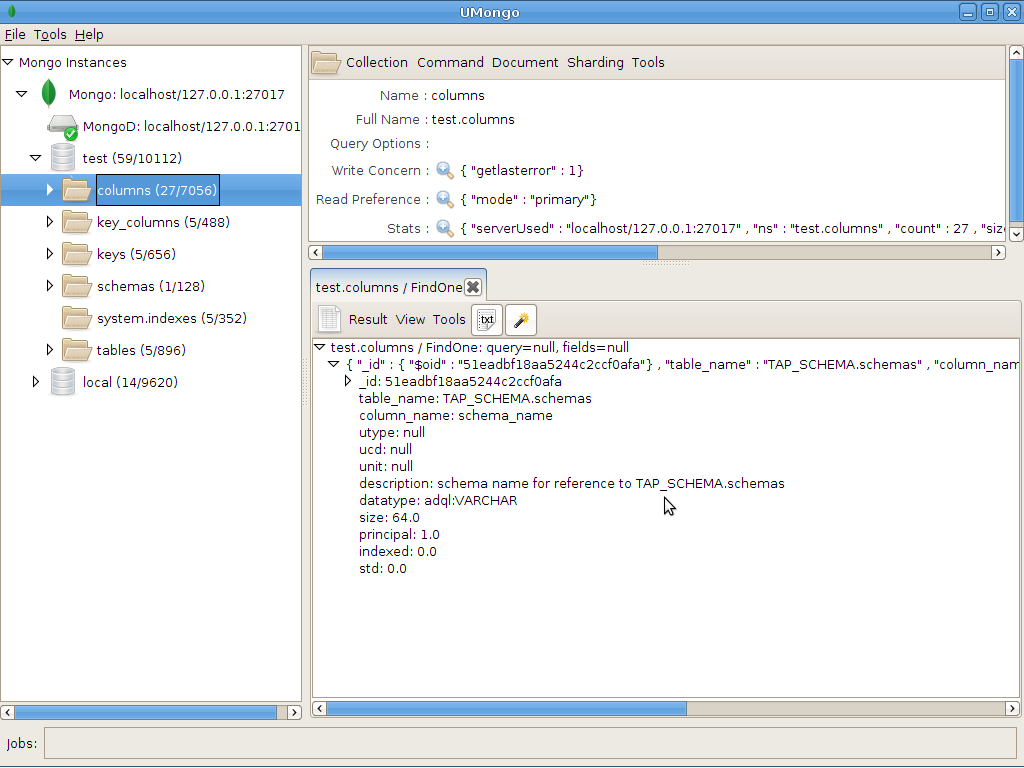
\includegraphics[width=11cm,height=8cm]{images/mongo_dia.png}
\caption{Tree View for Tap Schema in MongoVue}
\end{figure}


\subsubsection{Basic syntax quick guide SQL/Mongo}

\lstinputlisting[language=SQL]{/home/jose/Escritorio/TFM/src/sample01.sql}



\section{A FITS alternative with MongoDB}

A very important issue when working with FITS format is the great amount of possible key-value pairs in FITS headers. A possible solution for this problem could be use the features of MongoDB to translate FITS keywords into collections. So, we could create as much documents as needed, and storing them into MongoDB. Should we need to create supertypes of FITS headers, relations are also available in MongoDB through document linking (with no physical restriction in the sense of relational constraint). In this situation the schema flexibility means that we can model documents that share a similar structure but not enforced to have to same.

%TODO: ejemplo de conversión de fits a documentos de Mongo

\section{MapReduce in MongoDB}

MapReduce, developed by Google, is a programming model and its implementation for processing (\textit{e.g.} raw data from telescopes) and producing (\textit{e. g.} representations of graph structure of systems) huge amounts of data. As the runtime controls the partitioning of the input data, controlling the program execution across several hundred or thousands of nodes and even controlling machine failures, the developers with low or none expertise at all in parallel programming can take advantage of this model with a very low learning curve.\\

MapReduce, usually, is used to solve problems involving big size datasets, up to several petabytes. For this reason, this model is used in distributed file systems, like HDFS \footnote{For a full specification of this filesystem, go to \url{http://hadoop.apache.org/docs/stable/hdfs_design.html}}.\\

The MapReduce model allows to write a map function which takes a key/value pair, operates on it (performs object detection) and returns a new set of key/value pairs (source list). The reduce function then aggregates/merges all the intermediate data (builds an object catalog on a stacked source list). Many problems in astronomy naturally fall into this model because of the inherent parallelizability of many astronomical tasks.

\newpage

\lstinputlisting[language=Java]{/home/jose/Escritorio/TFM/src/map_reduce_01.js}
\chapter{Conclusions and future work} % (fold)
\label{cha:conclusions_and_future_work}

\section{Conclusions} % (fold)
\label{sec:conclusions}

\begin{itemize}

\item Relational approach are not always suitable for any problem. Non-relational systems are not cure-all, but it has been shown they can face some problems in a more efficient way (\textit{e.g.} MapReduce) and, in some situations, NoSQL can be a complement for existing RDBMS.

\item Any new proposal should be inside Virtual Observatory frame.

\item NoSQL database systems, specially -not exclusively- those document-oriented can reduce system analysis and design and can also succeed in boosting the performance of data management.

\end{itemize}

% section conclusions (end)

\section{Future work} % (fold)
\label{sec:future_work}

\begin{itemize}

\item Focusing in a workgroup inside Virtual Observatory instead of treating several aspects.

\item The use of formal metrics (CoCoMo, Function Point Analysis, etc.) to plan the software design and development and the costs involved.

\item Benchmarks support in order to obtain accurate data in performance improvements.

\item Deciding which language to use to connect the selected DBMS.

\end{itemize}

% section future_work (end)

% chapter conclusions_and_future_work (end)




\appendix
\chapter{Getting and installing MongoDB}


\begin{itemize}

\item Go to \url{http://www.mongodb.org/downloads} and select our OS version. Download it and decompress.
\item Supposing we are in a Linux box and that we are using the latest release (in June 2013) execute the following command: \begin{verbatim}./mongod --rest --dbpath /opt/mongodb-linux-i686-2.4.5/bin/data/db/ \end{verbatim}                                                                                                     
\item The server is now listening and waiting for connections, by default, in port 27017. As we have used the \textit{--rest} modifier, we can point our browser to \url{http://localhost:28017} for http diagnostic access.

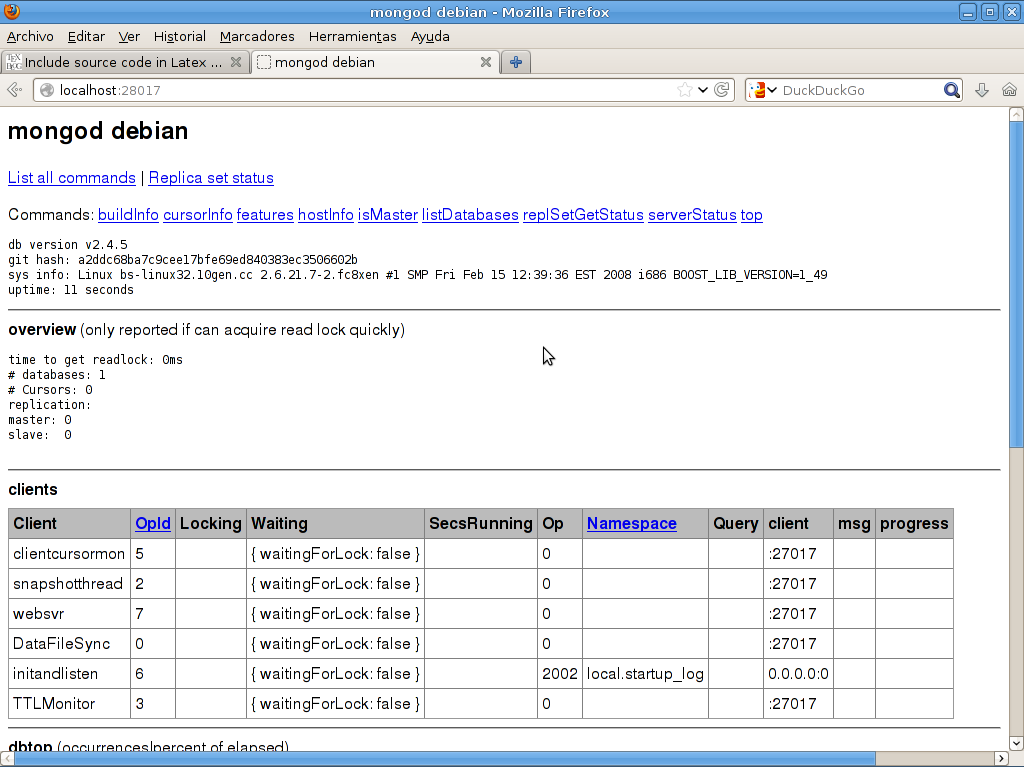
\includegraphics[width=11cm,height=8cm]{images/mongo_webconsole.png}

\end{itemize}
\chapter{Configuring Eclipse and NetBeans for Java/Mongo development}

\begin{itemize}
\item Go to \url{http://central.maven.org/maven2/org/mongodb/mongo-java-driver/} and choose the right version.
\item In Eclipse, just start a new project \textbf{File - New - Java Project}
\item Right-click in \textbf{Properties} and then \textbf{Java Build Path - Libraries - Add External JARs} 

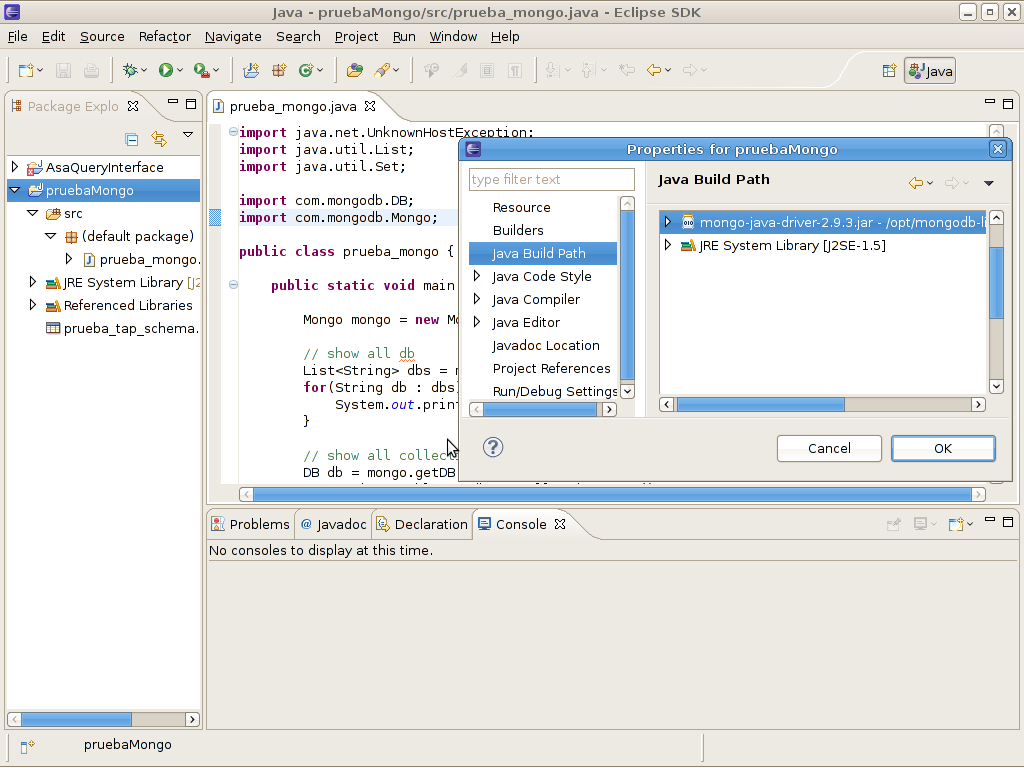
\includegraphics[height=8cm]{images/mongo_eclipse.png}

\item Import MongoDB methods, classed and interfaces as needed.
\item In NetBeans, start a new project \textbf{File - New Project - Java Application}
\item Right-click in \textbf{Libraries} and then \textbf{Add JAR/Folder} 

 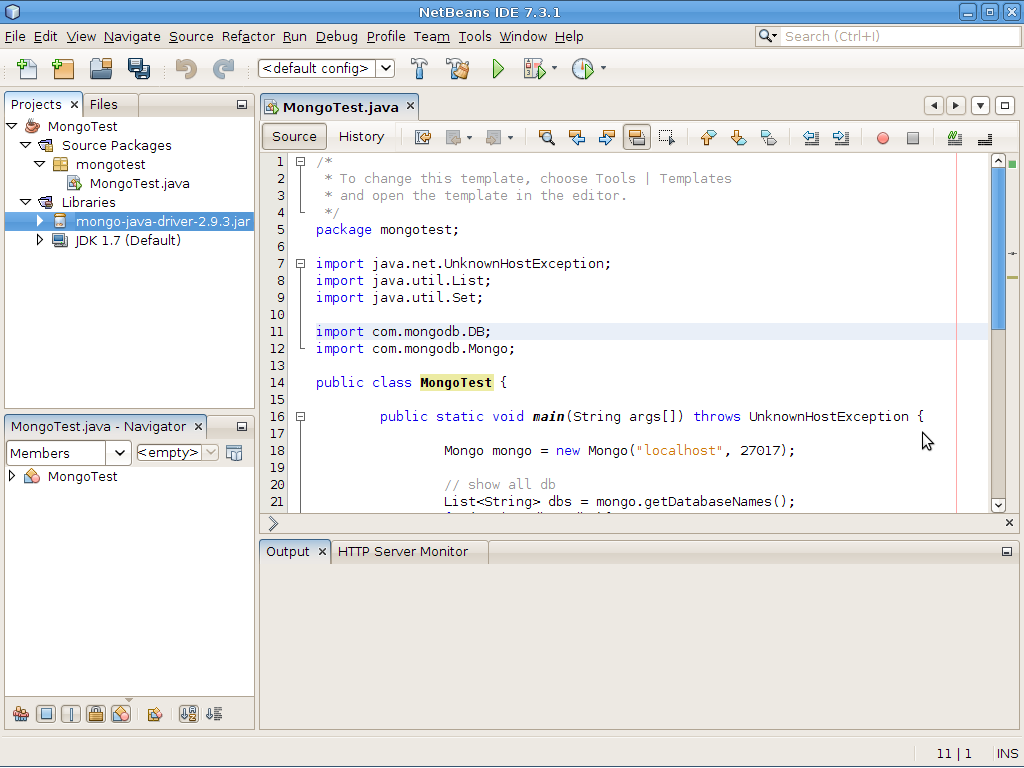
\includegraphics[height=8cm]{images/mongo_netbeans.png}

\item Import MongoDB methods, classed and interfaces as needed.
\end{itemize}


\nocite{*}
\bibliography{biblio}

\end{document}
